\section{Don’t Augment Me}\label{section:dont-augment-me-definition}

The first part of the experiments relies on the hypothesis that real-world augmentations, which do not cause any significant changes in the augmented image and also do not cause a model to change its prediction significantly, may cause an attribution method to produce significantly different attribution of the augmented image. To measure the difference in attributions quantitatively, I am going to use SSIM \cite{wang2004image} metric. Because quantifying a human visual perception cannot be measured with any known metric and is an active field of research, in addition to the SSIM metric, some of the attributions are going to be presented for qualitative measurement.

\subsection*{Procedure}

To be able to calculate the SSIM metric for the attributions, each dataset and method needs to have a maximum range calculated first. This requires an additional run through all images from the dataset through every model and used method to get a maximum value of attribution assigned by a method for a model. This value is used as a data range in SSIM for all attributions using the same method and model. Lists of calculated maximum attribution values are in appendix \ref{appendix:ssim-ranges}. This range is set for a given experiment and not going to be explicitly mentioned in every one of them unless it is relevant to the change in the setup.

\vspace{\baselineskip}

For an image from the test dataset, a set of augmentations will be applied. Augmentations are defined in Section \ref{section:augmentation}, and all of them are used. The original image, as well as augmented images, are then forwarded through a selected model to get a prediction score. If the prediction score of the augmented image is within the $threshold = 0.05$ that of the original image (non-augmented), then the augmented image is accepted for an attribution comparison. To get the attribution, both the augmented image and the original image are forwarded through a selected attribution method, and resulted attributions are the inputs to the SSIM function. The whole process could be defined as:

\begin{equation}
    SSIM_{x, x_i} = \begin{cases} SSIM(A(F, x), A(F, x_i)) & \text{if } |F(x) - F(x_i)| < 0.05 \\ \text{NaN} & \text{otherwise} \end{cases}
\end{equation}

Where $x$ is an original image, $x_i$ is an augmented image, $F$ is a model, $A$ is an attribution method. There is one exception from this equation, and it occurs when the augmentation is a \textit{rotation} (by any angle). The special case includes applying the same rotation to the attribution from the original image and can be summarized as:

\begin{equation}
    SSIM( R(A( F, x ), \theta), A( F, R(x, \theta)) ))
\end{equation}

The main condition ($|F(x) - F(x_i)| < 0.05$) is still in place, the $x_i$ is replaced by the $R(x, \theta)$, which uses a rotation function $R$ and the angle $\theta$. The same rotation $R$ is applied on the result from the attribution method $A( F, x )$. This fixes the issue of calculating the similarity of rotated attribution to the none rotated attribution. This special case is done under the assumption that rotation of the input image should cause the a similar rotation of the attribution for this image. Comparing attribution from the rotated image to the attribution from the original image would not make sense because the region which is the most important for a prediction is rotated by the $\theta$ angle.

\vspace{\baselineskip}

With all SSIM values calculated, each method will have a mean and the standard deviation value calculated. Additionally, mean and standard deviation values will also be calculated per augmentation. The first calculation should allow comparing the methods, and the second is going to be a supplementary check if there are any exceptions for particular augmentation. The qualitative comparison of the results will include visual rendering of selected examples (original images) along with all augmentations applied to that example. Because the amount of augmentations is far greater than it can be displayed in a comprehensive way, augmentations are going to be split into \textit{rotations} and \textit{filters}. \textit{Rotations} will include all available rotations \ref{section:rotations} (4 in total), and \textit{filters} will include everything except the \textit{rotations} (5 in total). For an example to be considered a valid example, all augmented versions of that example have to achieve class score within the $threshold < 0.05$ from the a score of the original image (non-augmented). This is a more restrictive criterion than the one used for each augmentation separately but removes any potential misinformation on which augmentation is used for valid or not.

\section{Can I Rely On You}\label{section:can-i-rely-on-you-definition}

The second part of the experiments is focused on testing the hypothesis that two of the most popular measures of XAI methods are not reliable when trying to use them to compare methods even within the same data domain. To be able to check if that hypothesis is true, we need to define how the measure should behave for it to be considered reliable.

\begin{definition}\label{def:reliability}
    Given an XAI method $A_1$ and $A_2$ and the measure $S(A)$, measure $S$ is considered reliable, when within the same data domain and model architecture, measures calculated for method $A_1$ always have the same relation to the measures calculated for the method $A_2$.
\end{definition}

\begin{figure}[h]
  \centering
 \begin{subfigure}{.3\textwidth}
    \centering
    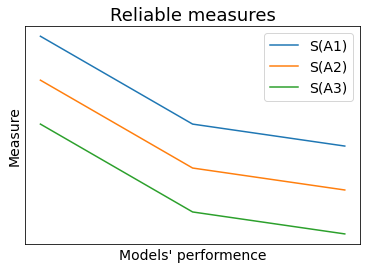
\includegraphics[width=\textwidth]{experiments/desc/rel1.png}
    \caption{}\label{fig:rel-measure-1}
\end{subfigure}
 \begin{subfigure}{.3\textwidth}
    \centering
    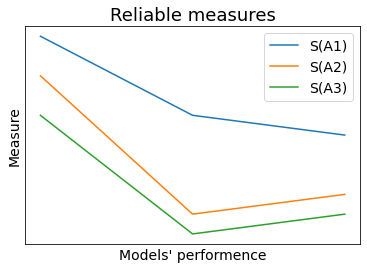
\includegraphics[width=\textwidth]{experiments/desc/rel2.png}
    \caption{}\label{fig:rel-measure-2}
\end{subfigure}
 \begin{subfigure}{.3\textwidth}
    \centering
    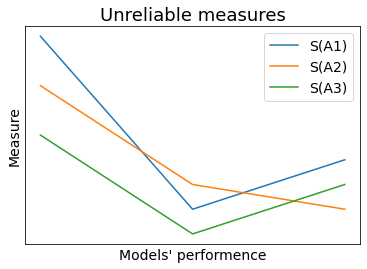
\includegraphics[width=\textwidth]{experiments/desc/unrel1.png}
    \caption{}\label{fig:unrel-measure}
\end{subfigure}

 \caption{An example of reliable measures (Fig. \ref{fig:rel-measure-1}, \ref{fig:rel-measure-2}) and unreliable measures (Fig. \ref{fig:unrel-measure})}\label{fig:reliable-measures-example}
\end{figure}

To illustrate definition \ref{def:reliability}, let us consider an example in Figure \ref{fig:reliable-measures-example}. Each chart represents a relation between the measure score and the models' performance (it could be $F1$ or any valid metric). The ideal measure is shown in Figure \ref{fig:rel-measure-1}, where the relation between values for different attribution methods ($A1$, $A2$, and $A3$) remain the same with the change of models' performance. Changes in the absolute value are not relevant here. The second example (Fig. \ref{fig:rel-measure-2}) is also a valid measure but not as ideal as the first one. Relation between values is changed, but the order of the values is always the same. The third example (Fig. \ref{fig:unrel-measure}) shows the behavior of the unreliable method. The relation between values is changing, and the order in which values for each method are presented is also changing. If there were only two methods in the third example ($A1$ and $A3$), we could assume the measure is reliable. That is the reason why when testing a given measure, we should use more data points.

\subsection*{Procedure}

To properly validate measure Infidelity (Section: \ref{section:infidelity}) and Sensitivity (Section: \ref{section:sensitivity}), each of them has to be tested on every trained model. That gives a total of $375$ different data points for the measure (5 XAI methods $\times$ 5 datasets $\times$ 5 train data fractions $\times$ 3 models). Each data point consists of measures for every sample from the train dataset used for a particular model.

\begin{remark}
The Integrated Gradients (Section \ref{section:ig}) method is not used in this experiment because computing the value of Sensitivity for this method requires more than 11GB of memory.
\end{remark}

Infidelity uses a Gaussian noise with a $\mu = 0$ and $\sigma = 0.003$ to perturb images. Sensitivity creates $10$ perturbed images with the help of the function that samples uniformly random from the $L_{Infinity}$ ball with $0.02$ radius. The results from each data point are processed, and the mean and standard deviation values are calculated. 